\chapter {Preliminary Work}

\section {Preliminary Experiments}

	\subsection {What Concentration of Sulfuric Acid to use?}

Originally I planned to use 10 cm$^3$ of sulfuric acid and then add 30 cm$^3$ of distilled water, but I found that this was too slow. Therefore I decided to use 40 cm$^3$ of sulfuric acid and not dilute with any further water. From my experiments i decided that 2 molar sulfuric acid would be the starting concentration for my range of experiments without a catalyst.









	\subsection{Which Form of Zinc to use?}

I ordered two types of zinc in order to compare the use of them. These two forms were granulated and powdered Zinc. Below is a picture of the granulated zinc.

\begin{figure}[H]
    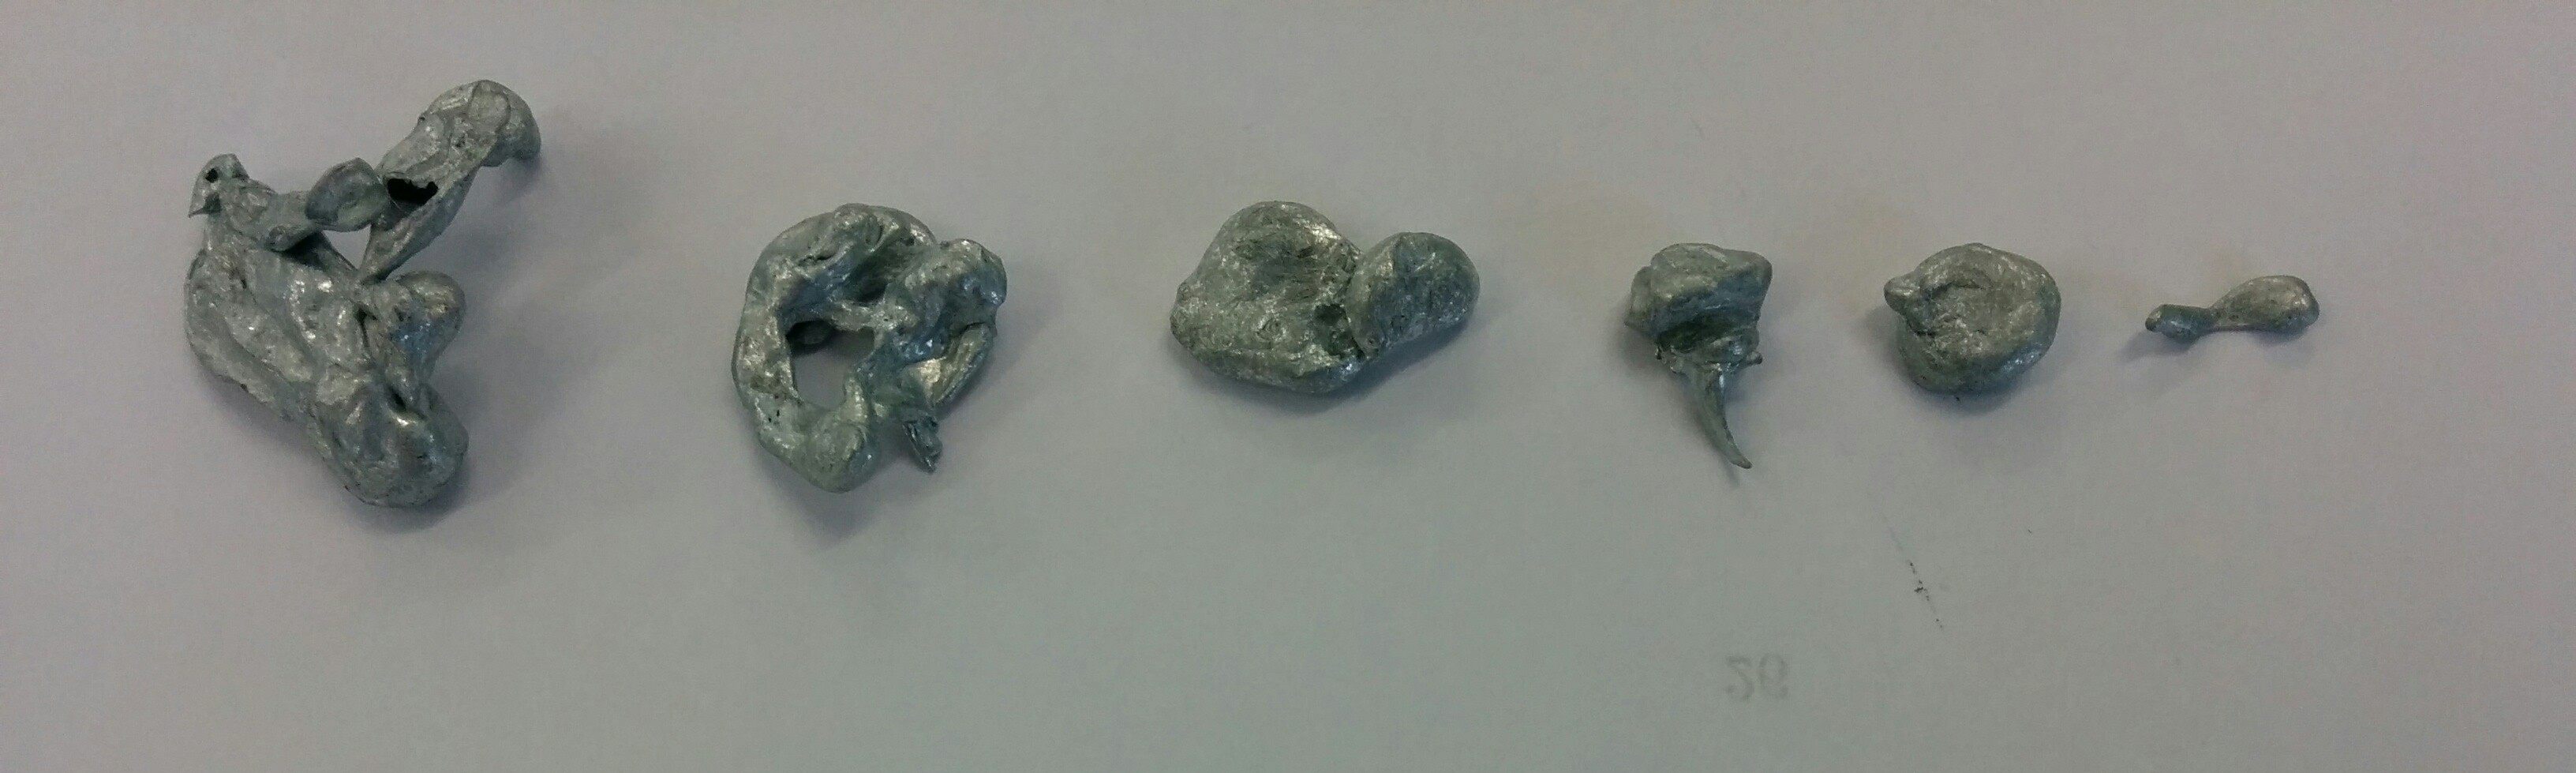
\includegraphics[width=\textwidth]{./preliminarywork/images/GranulatedZinc.jpg}
    \caption{Granulated Zinc.} \label{fig:Granulated Zinc}
\end{figure}

As you can see the sizes of the chunks of the Zinc vary dramatically. This meant that I could not accurately measure 1.0 g of Zinc using the granulated Zinc, and also the varying surface area to volume ratio would cause the experiment to not be accurate and produce unreliable results. The powdered Zinc was extremely finely grinded which allowed for a more reliable surface area to volume ratio, which as discussed in the chemical ideas section has an impact on the rate of reaction.



	\subsection{Inverted Burette Method vs Gas Syringe Method} 

To work out which method would be best to carry out my experiment, I decided to carry out the two most viable methods. From this experiment I decided that the method which gave the most reliable results would be the method I used to carry out my actual experiment. For this experiment I decided to measure the volume of Hydrogen gas produced over a 5 minute period, with 1.0 g of powdered Zinc and 40 cm$^3$ of 2.0 molar Sulfuric acid. My results are shown below for both method.

\begin{figure}[H]
    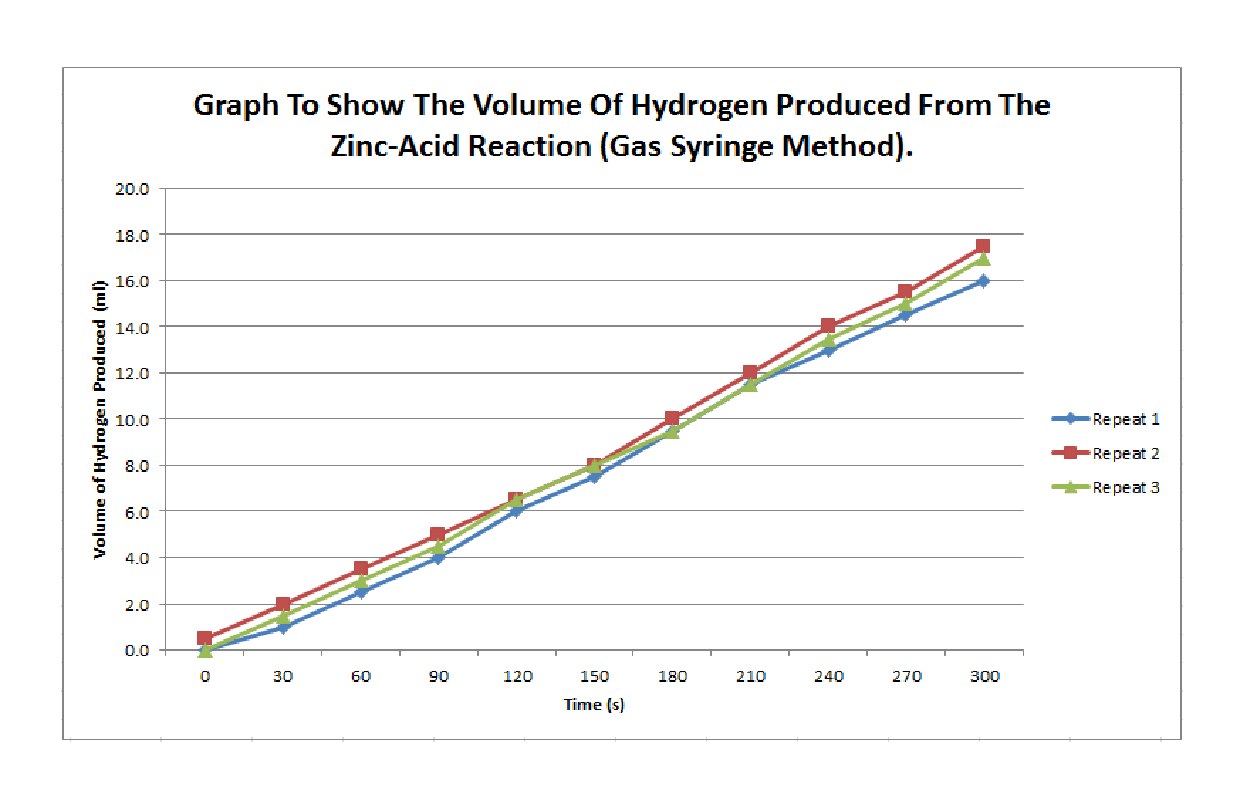
\includegraphics[width=\textwidth]{./preliminarywork/Graphs/GasSyringe.pdf}
    \caption{Gas Syringe Method Graph} \label{fig:Gas Syringe Method Results}
\end{figure}

Above shows the graph of my results for the gas syringe method.This shows that the average volume collected was 16.7 ml of gas and the average range was only 1.0 ml. For the raw data table which I used to analyse this from please look at Figure \ref{fig:GasSyringeRawData} on page \pageref{fig:GasSyringeRawData} in the preliminary work section appendix.




\begin{figure}[H]
    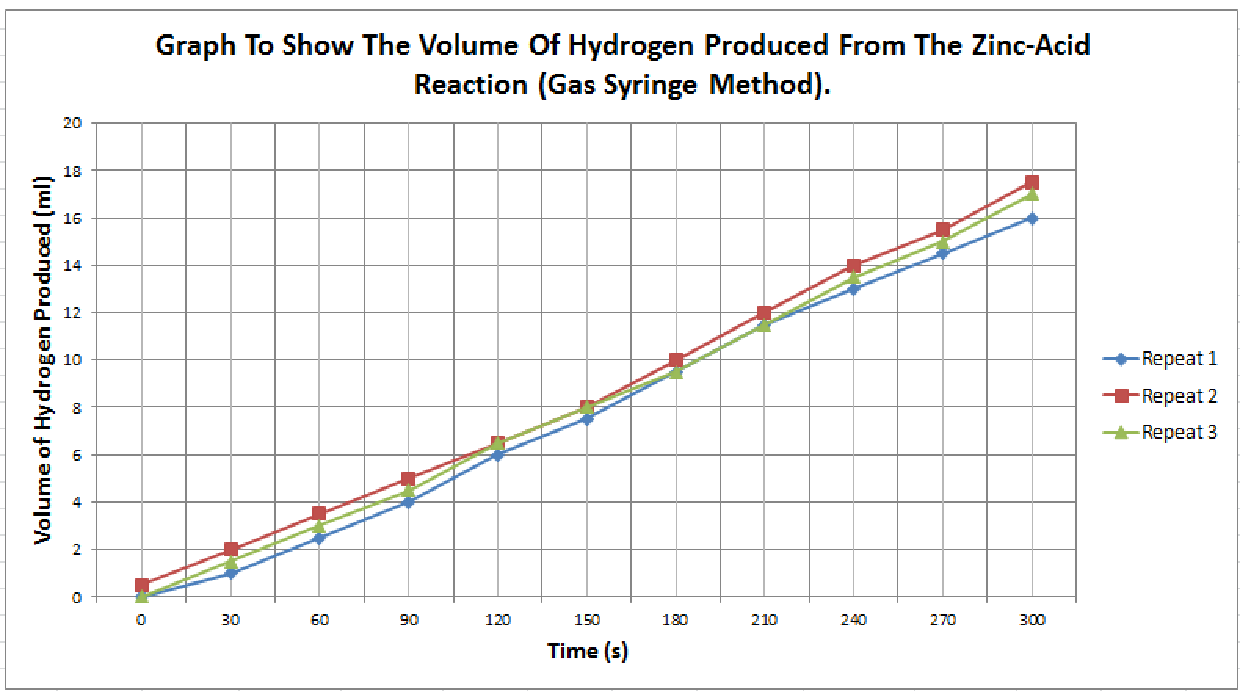
\includegraphics[width=\textwidth]{./preliminarywork/Graphs/Burette.pdf}
    \caption{Burette Method Graph} \label{fig:Burette Method Results}
\end{figure}

Above shows the graph of my results for the burette method. This shows that the average volume collected was 11.87 ml and the average range was 2.20 ml. For the raw data table which I used to analyse this from please look at Figure \ref{fig:BuretteRawData} on page \pageref{fig:BuretteRawData} in the preliminary work section appendix.



In conclusion I decided that the gas syringe method was more reliable as the average range was only 1.0 ml in comparison to the inverted burette method which produced a significantly larger range of 2.2 ml.  The burette method also collected significantly less hydrogen. I believe this occurred as the Hydrogen was being passed through a water medium, therefore some of the gas was absorbed into the water. This also was a factor that made me chose the gas syringe method over the burette method, as in the gas syringe method the hydrogen produced does not pass through a water medium and therefore would not dissolve into it. Although the burette read to two decimal places instead of one, the actual results produced by the burette method appeared to be unreliable, therefore I have chosen to use the gas syringe method for my experiment.




	\subsection{Measuring the Temperature of the Reaction}

As toom temperature varies from day to day I decided to measure the the temperature at the beginning of the day of experiments and as the Zinc-Acid reaction is an exothermic reaction, I knew that the temperature of the solution would increase as time went on. It turned out that all of the days that I carried out my experiments the solutions were all at the same temperature. They also produced the same temperature increase of 1$\circ$C. This graph is shown below.


\begin{figure}[H]
    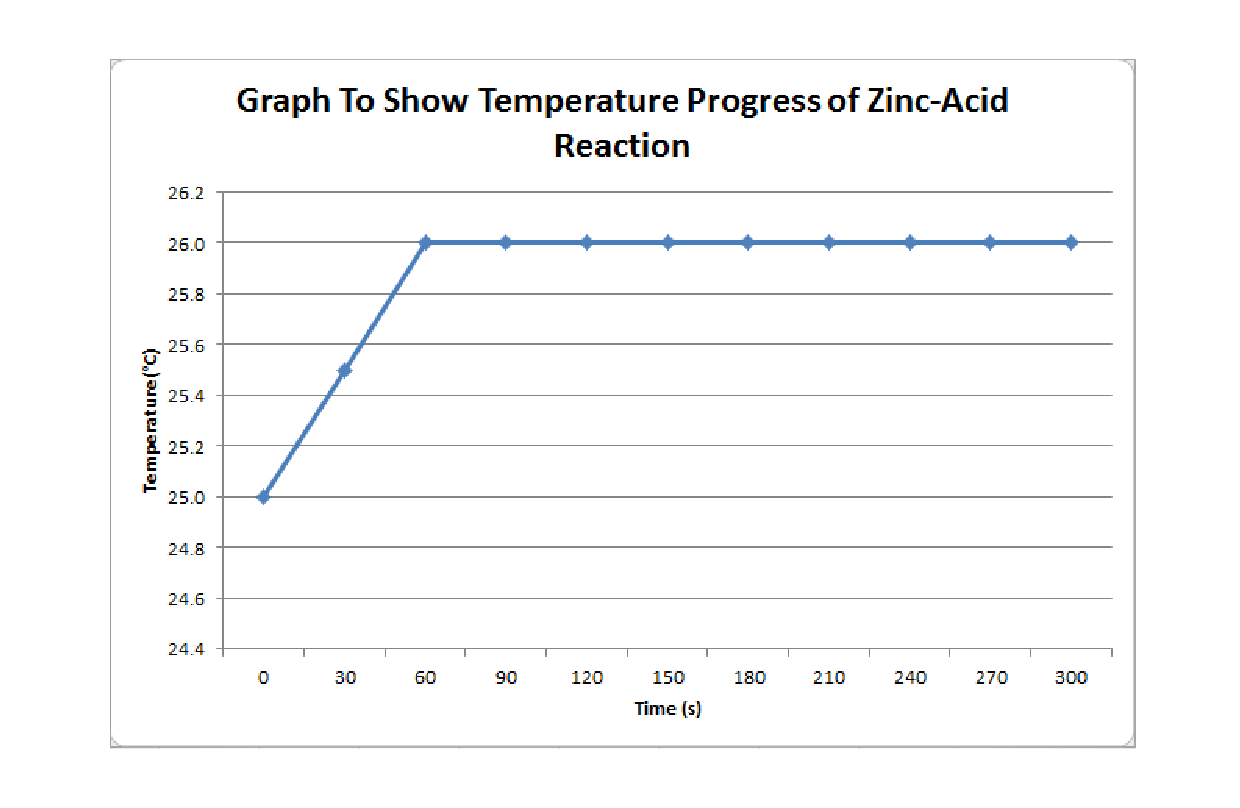
\includegraphics[width=\textwidth]{./preliminarywork/graphs/Temperature.pdf}
    \caption{Graph To Show The Temperature Progress of the Zinc-Acid Reaction.} \label{fig:Temperature Graph}
\end{figure}

Below you can see the apparatus that I used in order to measure the temperature of the reaction.

\begin{figure}[H]
    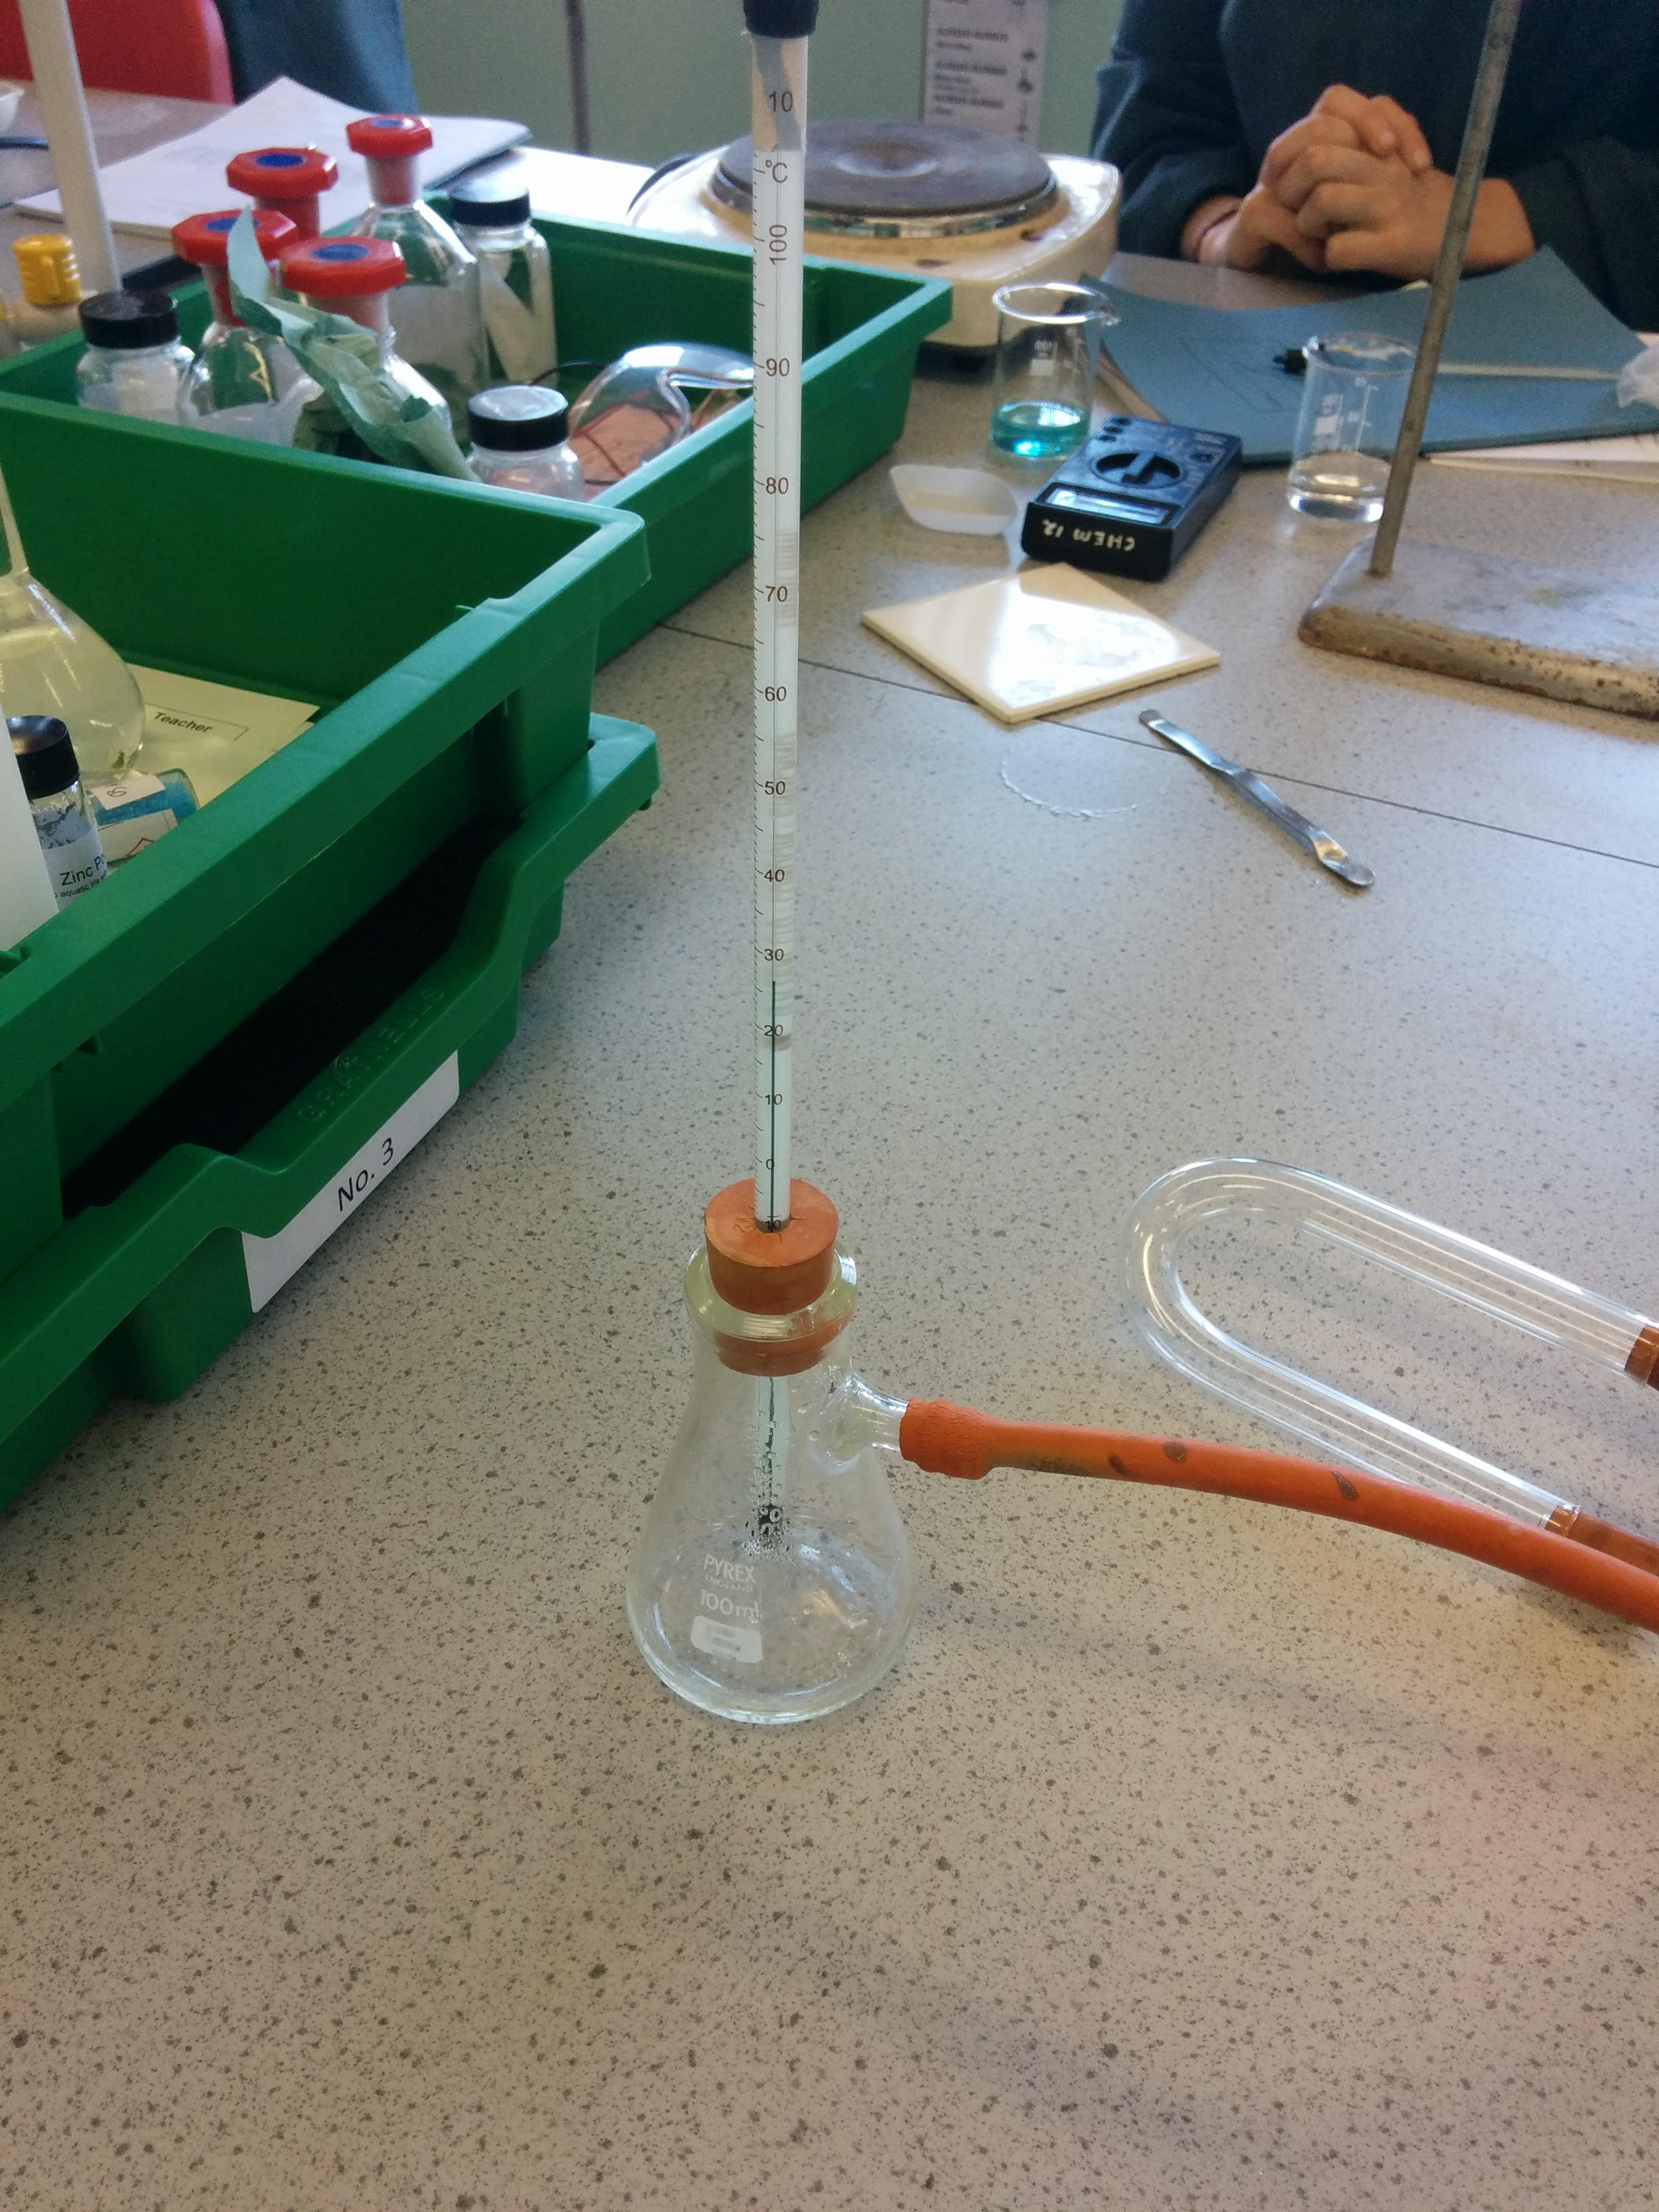
\includegraphics[width=\textwidth]{./preliminarywork/images/ThermometerSetUp.jpg}
    \caption{Thermometer set-up.} \label{fig:Thermometer Set-Up}
\end{figure}

My set-up involved the bung in the conical flask being modified to have a hole in it to stick a thermometer in it. Although the set-up allowed me to measure the temperature of the reaction, I decided not to measure the temperature of every experiment series as the hole in the bung caused the set-up to not be air tight. This meant that I would not collect the correct amount of hydrogen produced from the reaction. Below the two images show the set-up being in place, but when the gas syringe is pushed in, an excess amount of volume is lost.

\begin{figure}[H]
    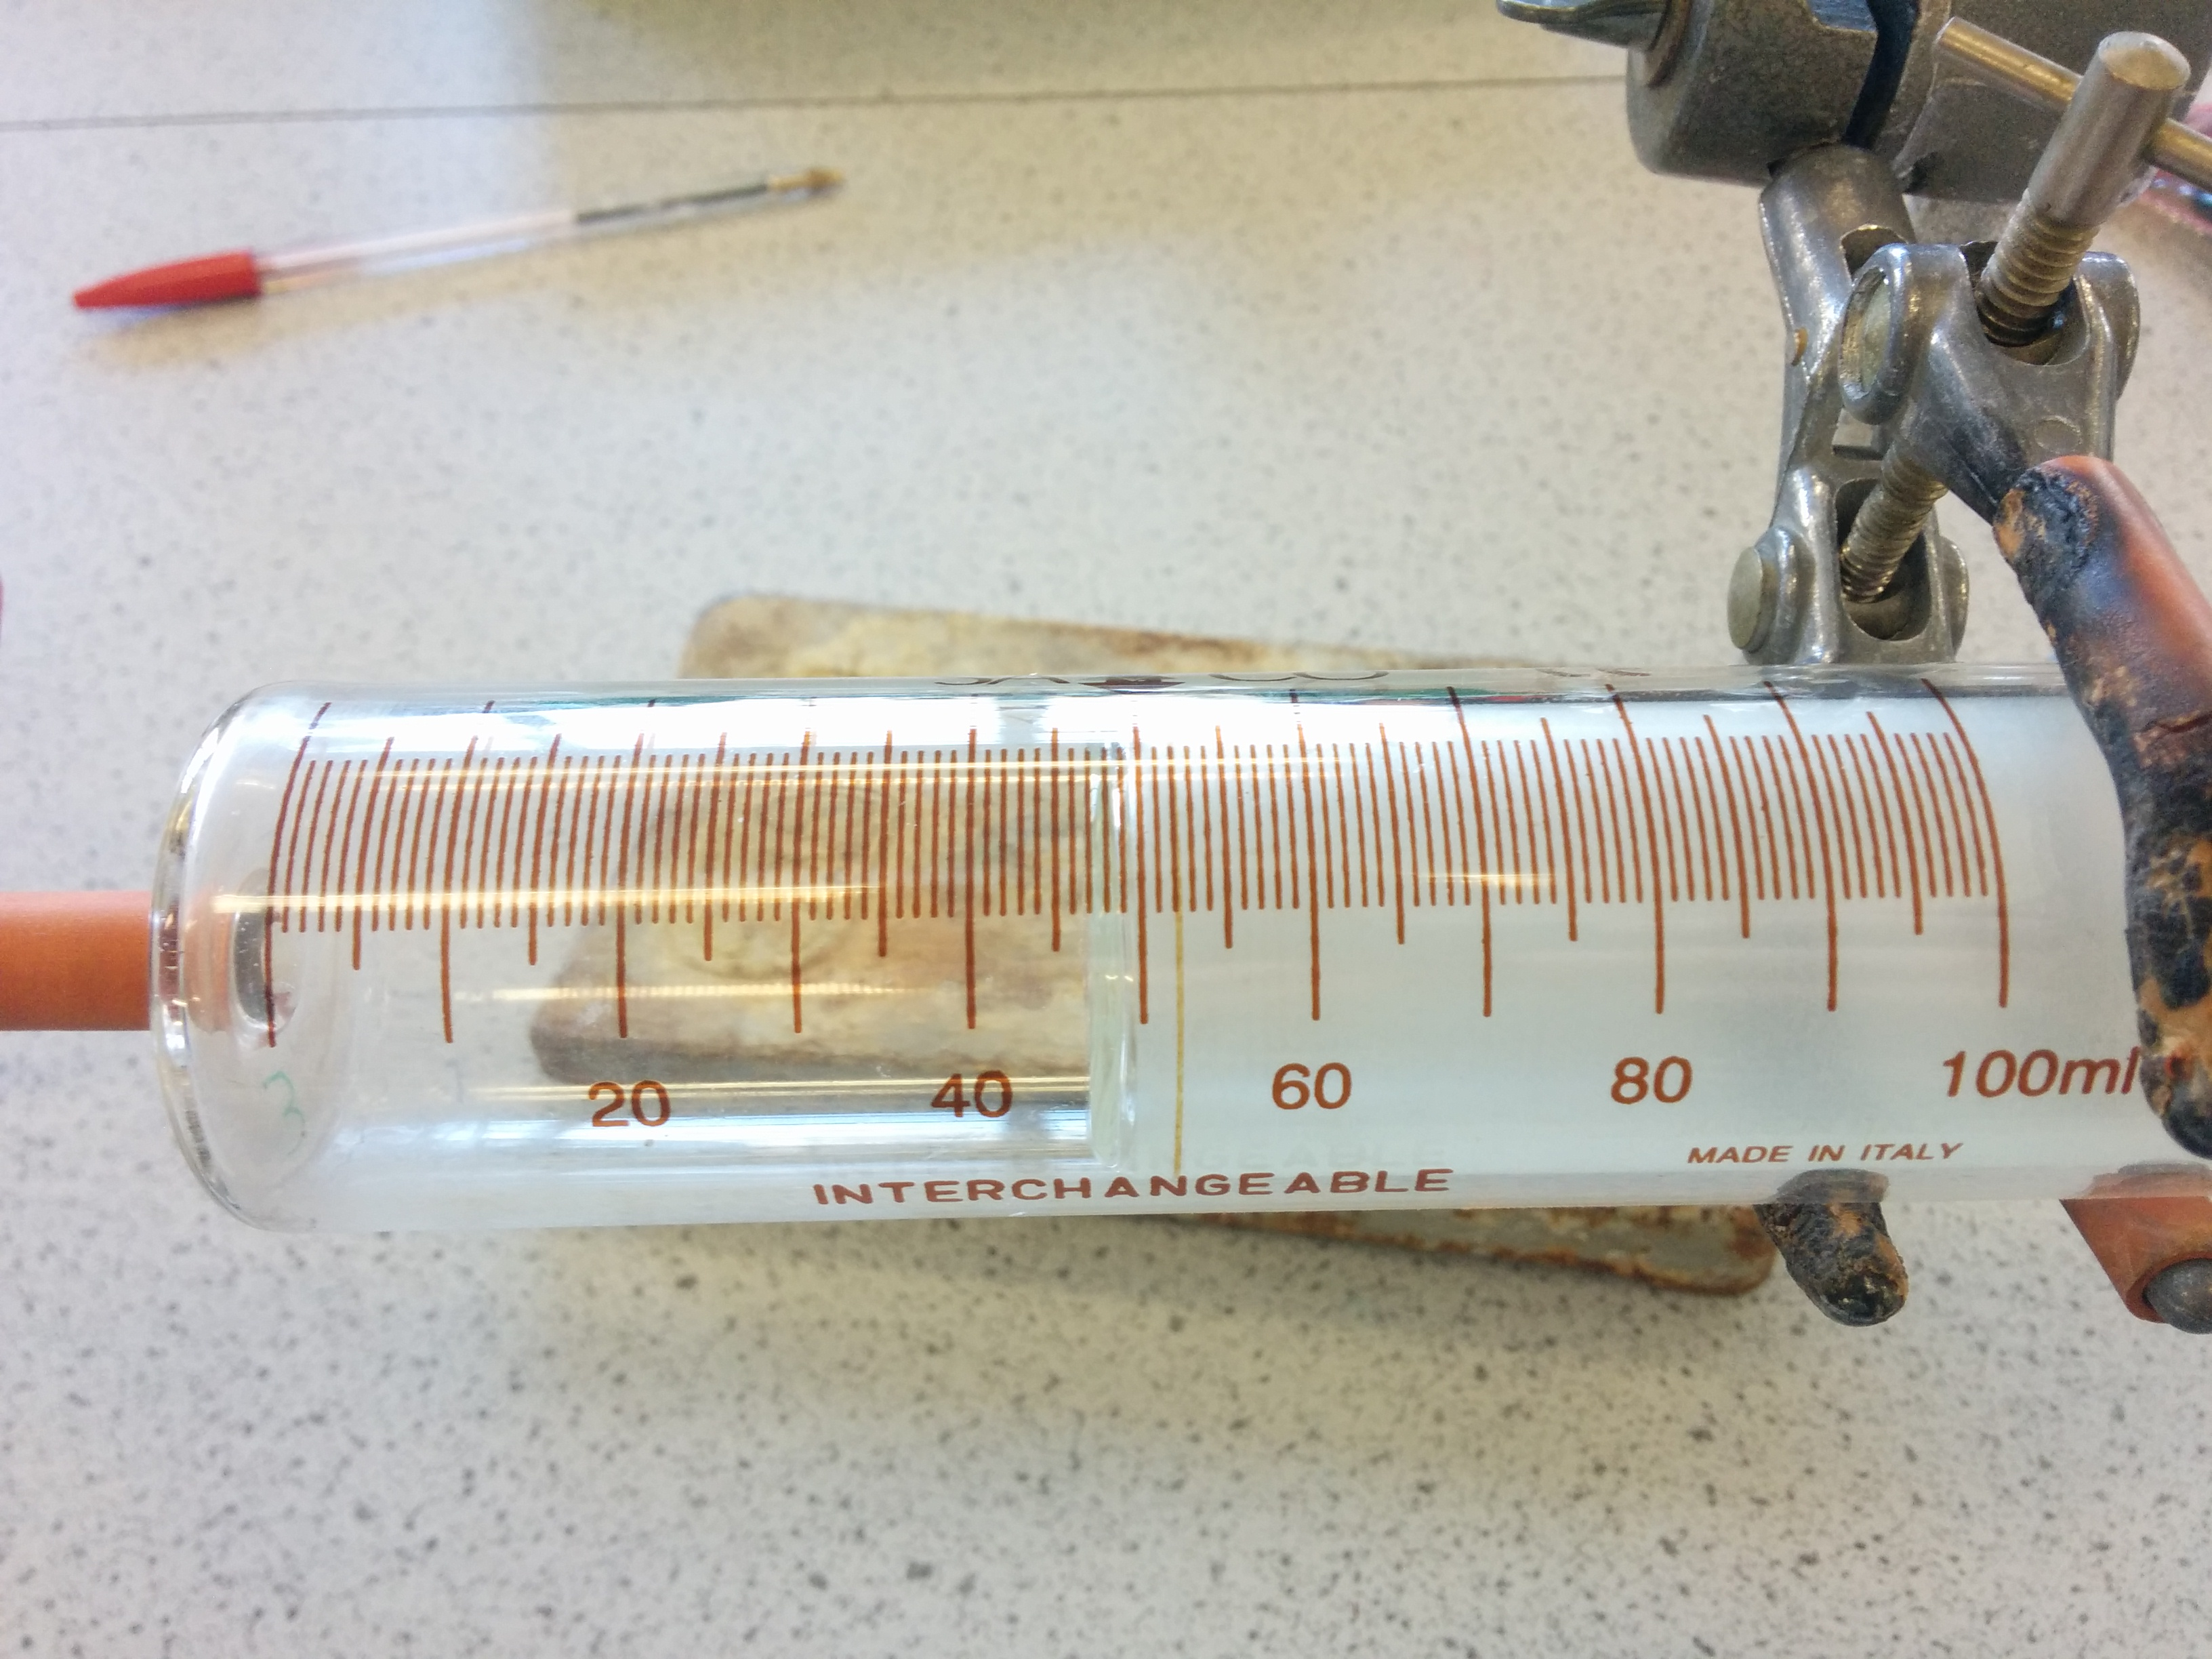
\includegraphics[width=\textwidth]{./preliminarywork/images/BeforePush.jpg}
    \caption{Before Pushing The Gas Syringe.} \label{fig:BeforePush}
\end{figure}

The image above shows the value of 52.0 ml of gas before pushing the gas syringe in.

\begin{figure}[H]
    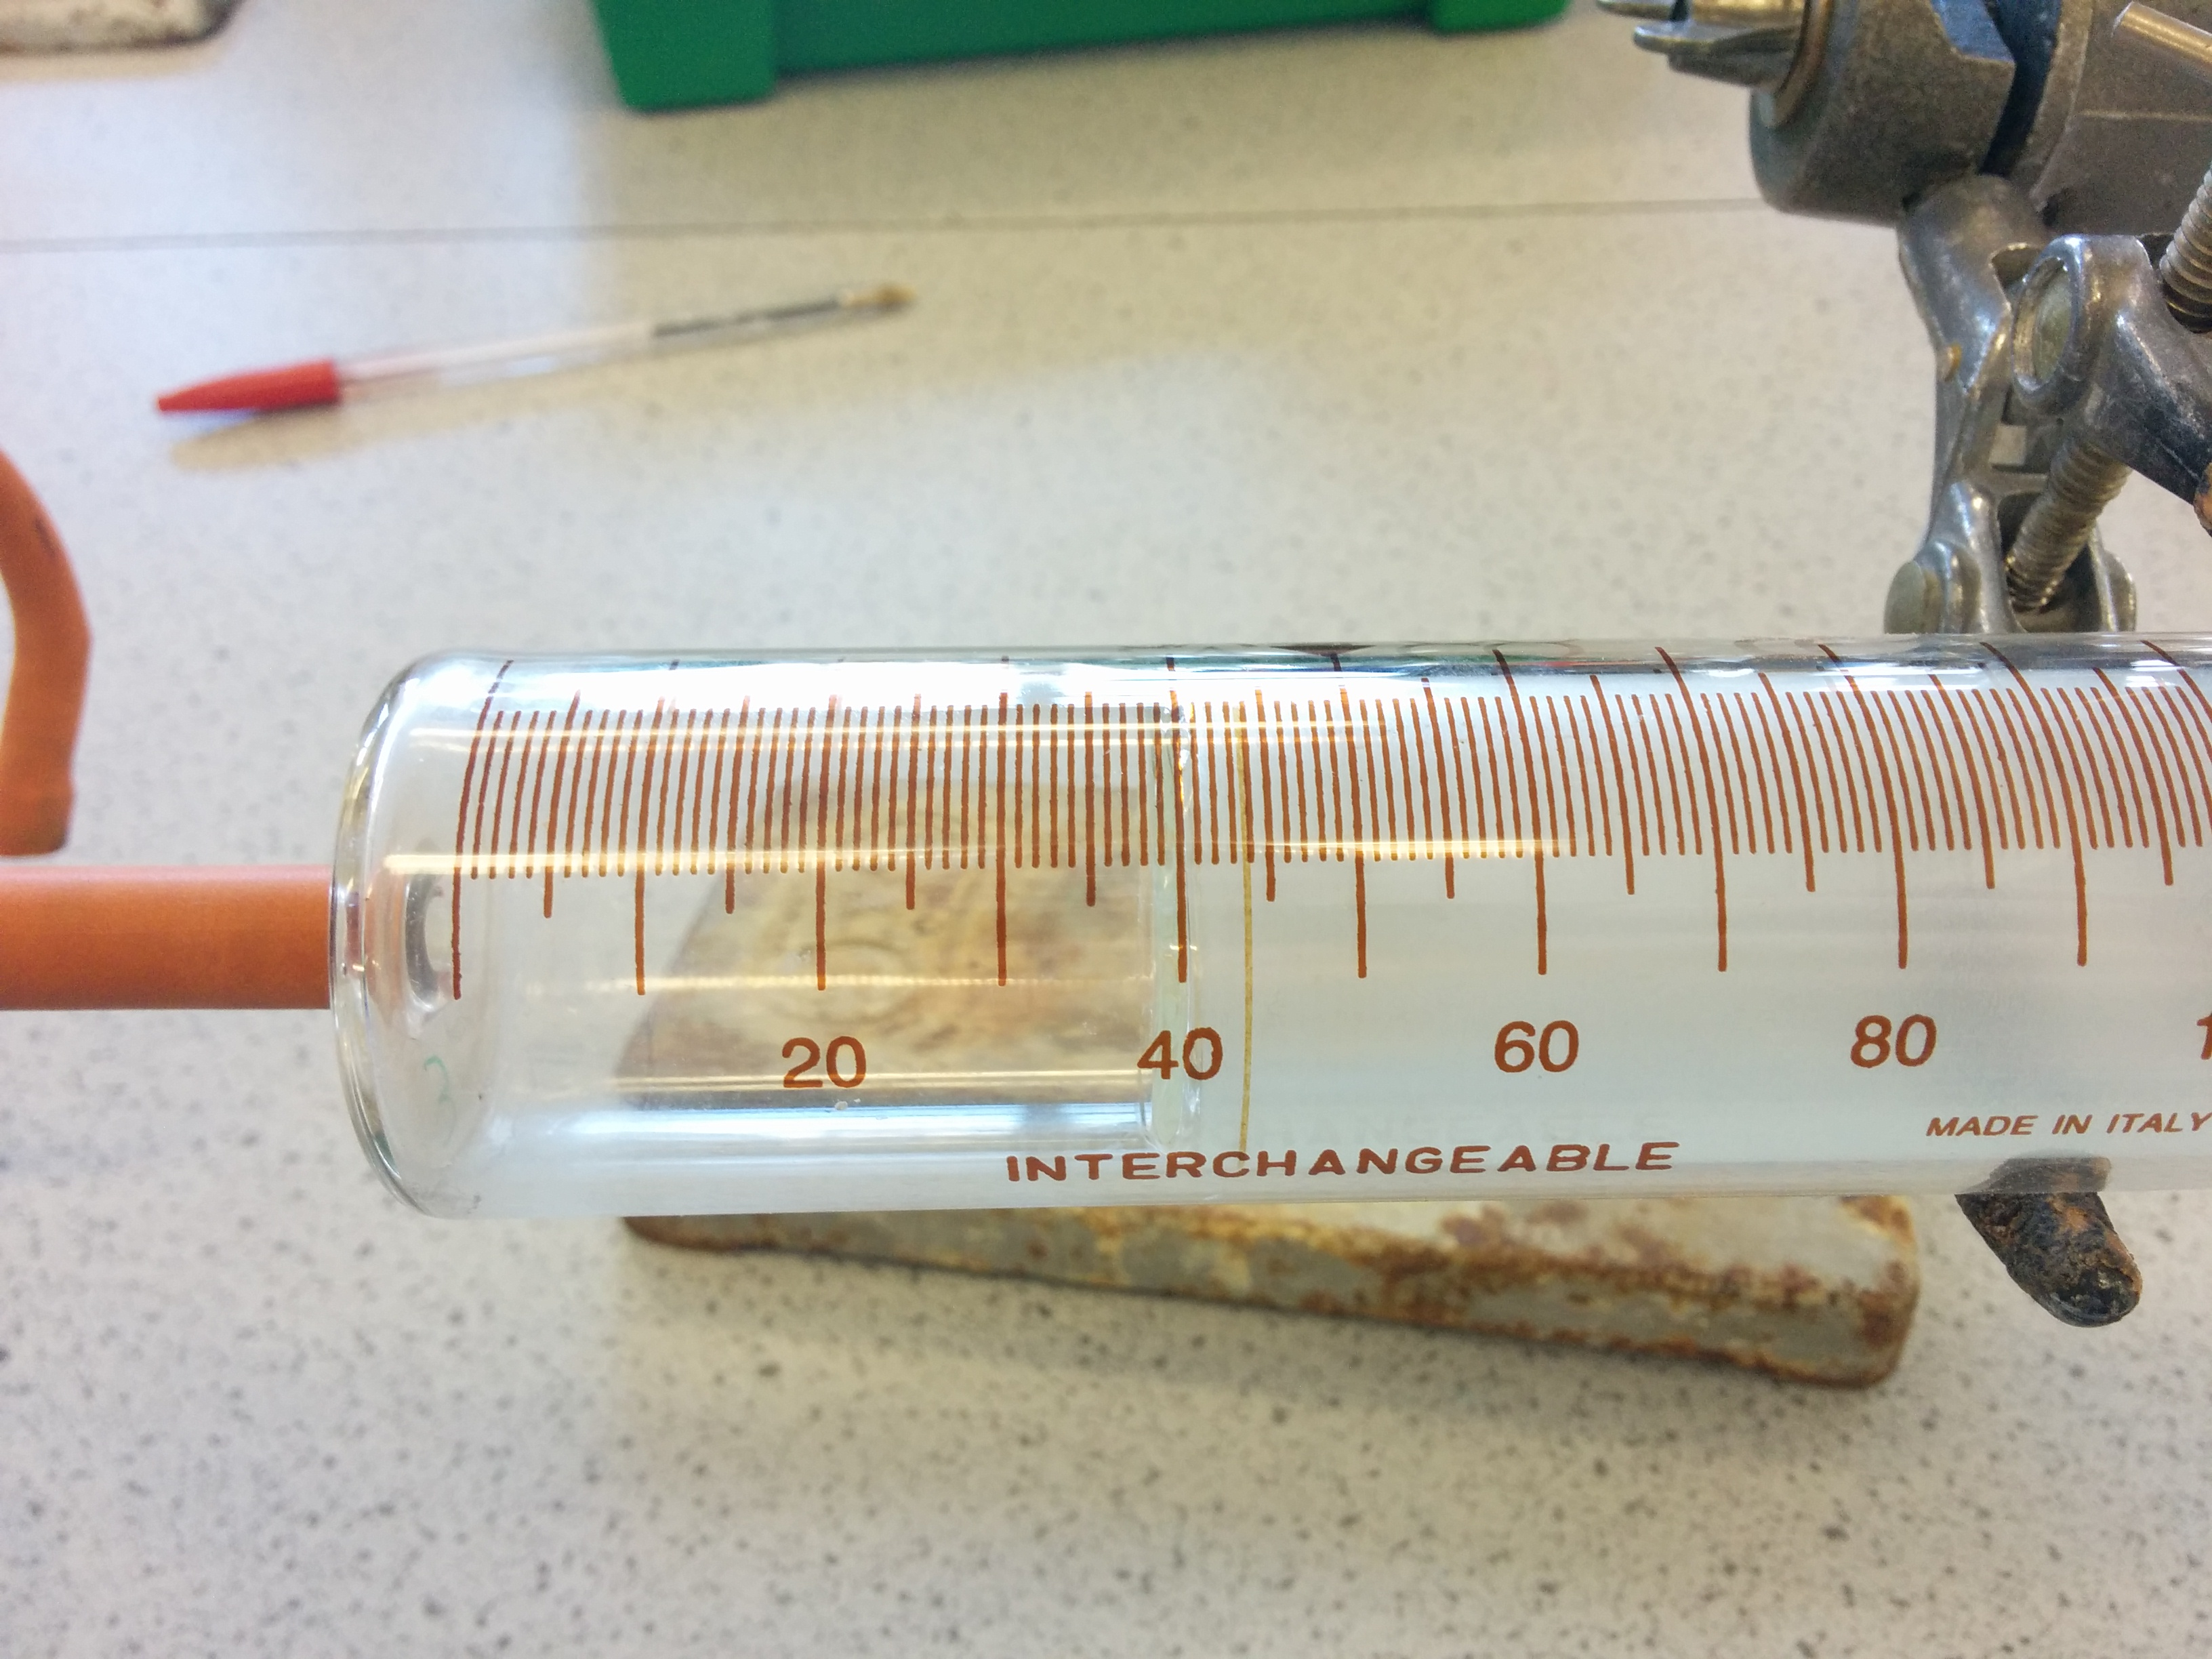
\includegraphics[width=\textwidth]{./preliminarywork/images/AfterPush.jpg}
    \caption{After Pushing The Gas Syringe.} \label{fig:AfterPush}
\end{figure}

The image below shows the value of 44.0 ml of gas after pushing the gas syringe in. This means that a total of 8.0 ml of gas was lost from pushing the gas syringe in, this indicates a significant gas leak. Therefore I used a complete bung and this shows to be air tight, as when it was pushed in the gas syringe returned to the same value. For the raw data table which I used to analyse this from please look at Figure \ref{fig:TemperatureRawData} on page \pageref{fig:TemperatureRawData} in the preliminary work section appendix.



\section {Techniques}

Through carrying out my preliminary work, I found out a number of techniques that I could use to increase the accuracy and validity of my results.

	\subsection{Order of Adding Reactants}

Through my preliminary experiments I found that adding the sulfuric acid first then the zinc caused the zinc to have a tendency to form clumps, thus decreasing the volume of Hydrogen produced due to a decreased surface area. Therefore in my real experiment I will add the Zinc first then pour the sulfuric acid into the conical flask after.

	\subsection{Spreading the Zinc}

As Zinc powder has a tendency to form clumps when a solution is added, I decided to spread the zinc across the bottom of the conical flask before adding the sulfuric acid. This reduced the clumping effect of the Zinc powder and as I spread the zinc in the same way every time, it led to a more reliable and accurate experiment.

	\subsection{Cleaning the Gas Syringe}

I found that sometimes (due to others using the same equipment in between me) the gas syringe had something in it which caused it to get stuck at certain points. Because of this I decided to clean out the gas syringe every time I used it to reduce the friction and chance of it getting stuck.


\section{Preliminary Work Raw Data Appendix}

\textbf{Gas Syringe Method Raw Data}\begin{figure}[H]
    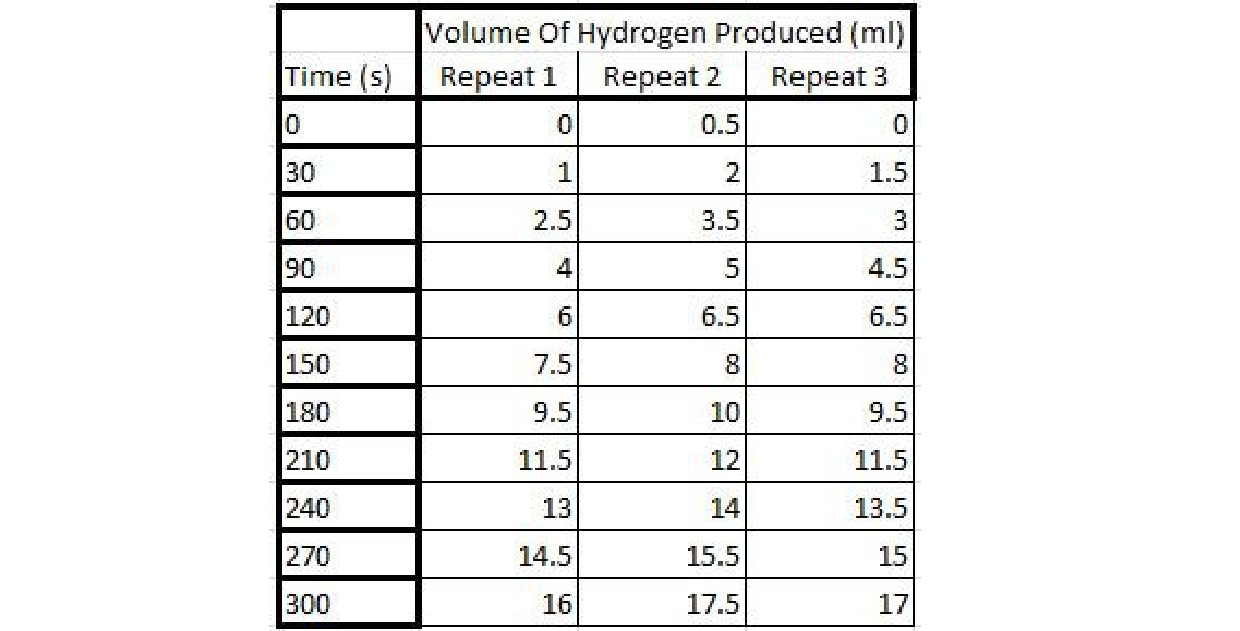
\includegraphics[width=\textwidth]{./preliminarywork/images/GasSyringeRawData.jpg}
    \caption{Gas Syringe Method Raw Data} \label{fig:GasSyringeRawData}
\end{figure}

\textbf{Burette Method Raw Data}\begin{figure}[H]
    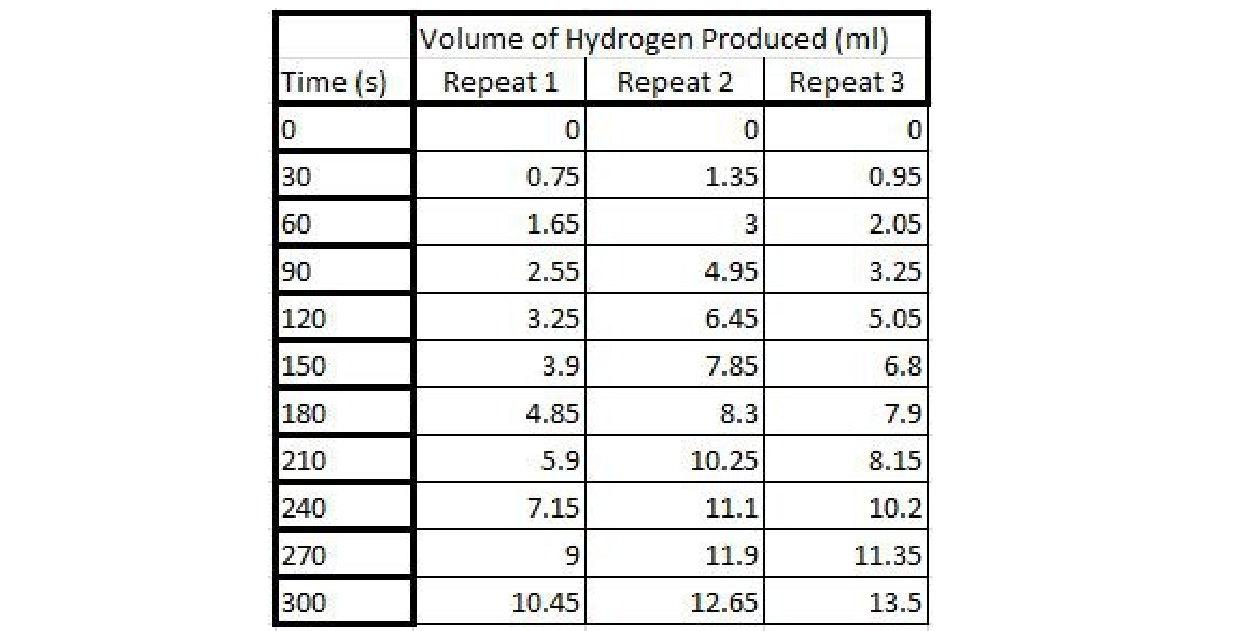
\includegraphics[width=\textwidth]{./preliminarywork/images/BuretteRawData.jpg}
    \caption{Burette Method Raw Data} \label{fig:BuretteRawData}
\end{figure}

\textbf{Temperature Experiment Raw Data}\begin{figure}[H]
    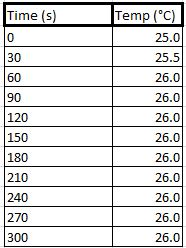
\includegraphics[width=\textwidth]{./preliminarywork/images/TemperatureRawData.jpg}
    \caption{Temperature Raw Data} \label{fig:TemperatureRawData}
\end{figure}

	